\chapter{Examples}
\label{chap:examples}

In this chapter we will introduce an example scenario of a process and how the resulting Code of the transformation look like.

\section{The Model}
The example process model is based on a scenario taken from the actual topic \textit{electromobility}. The scenario includes a choreography between a MobileApplication, started by a user wanting to reserve a taxi and a number of ETaxi-applications installed in electronic taxis. Figure \ref{fig:usecase} shows the usecase model of the \textbf{requestTaxi} process. 
\begin{figure}[h]
	\centering
		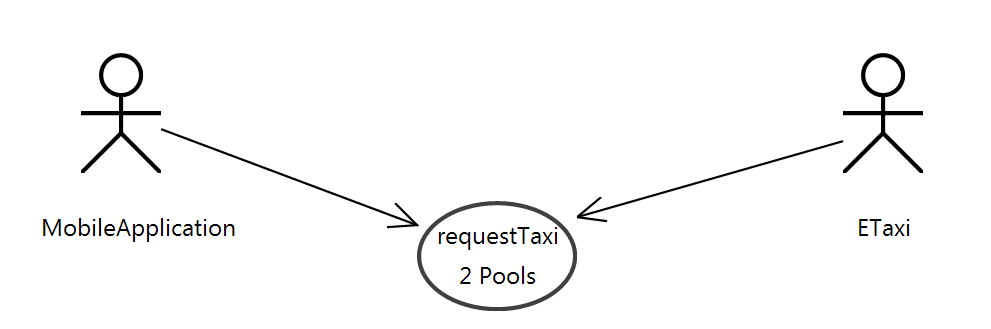
\includegraphics[width=0.8\textwidth]{images/example/usecase.png}
	\label{fig:usecase}
	\caption{Use case model}
\end{figure}

In Figure \ref{fig:payloads} we can see some data types included in the process which represents the information exchanged in the communication between both Pools (the payload of the implementing MessageChannel). At the moment Data types can not be defined in the model. They can only be included, the transformation will assume that the classes exists and they will be imported by the generated agent bean. Because they will be wrapped in a JiacMessage, the payloads has to implement the IFact interface.
\begin{figure}[h]
	\centering
		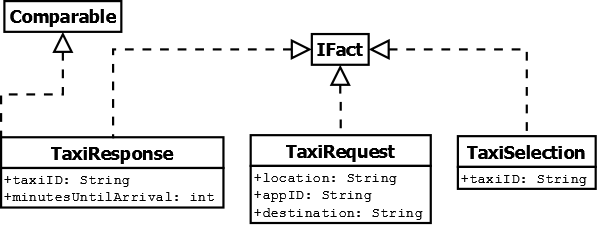
\includegraphics[width=0.8\textwidth]{images/example/payloads.png}
	\label{fig:payloads}
	\caption{Payloads included in the MessageChannel}
\end{figure}

\newpage
\subsection{The scenario}
\textbf{Mobile Application}\\
The process starts with a user requesting a taxi with the service provided by the mobile application. The service will then send a request to all ETaxis by sending informations about the user's location, application ID and the destination. Within 30 seconds after sending the request, the mobile application will collect responses from available ETaxis containing informations about the taxi ID and the estimated time needed by the taxi to arrive at the guest's current location. While receiving these responses, the mobile application will save the best response according to the minimum estimated time. After 30 seconds it will check whether a taxi is available, in which case it will send a notification to all taxis about which taxi is selected and then the process will end, passing the selected taxi's ID to the user. If no responses are received, it will notify the user that no taxi is currenty available. 


\textbf{ETaxi}\\


\begin{sidewaysfigure}
	\centering
		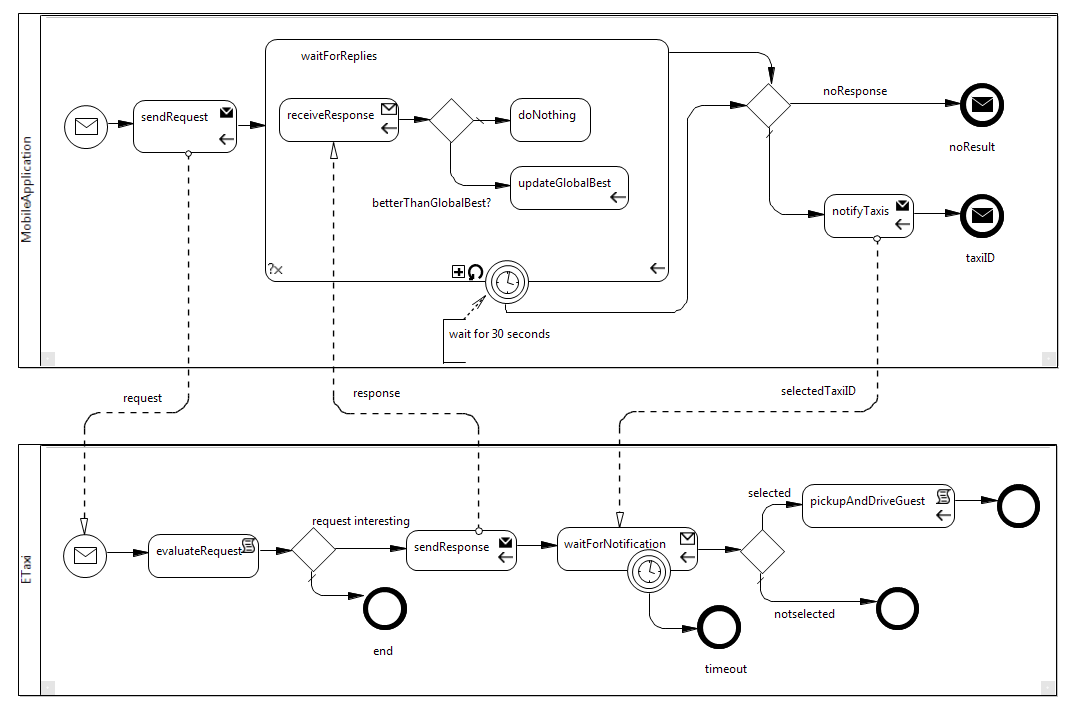
\includegraphics[width = 0.9\textwidth]{images/example/requestTaxi.png}
	\label{fig:example}
	\caption{Business Process Diagram - requestTaxi}
\end{sidewaysfigure}

\newpage
\section{The generated Agent Beans}
\textbf{1. MobileApplication\_requestTaxi}\\

\begin{lstlisting}[language=java, caption= Generated Agent Bean - MobileApplication\_requestTaxi]
package mobileapplication;

import de.dailab.jiactng.agentcore.action.AbstractMethodExposingBean;
import de.dailab.jiactng.agentcore.action.scope.ActionScope;
import input.TaxiResponse;
import input.TaxiRequest;
import input.SelectedTaxi;
import de.dailab.jiactng.agentcore.action.Action;
import de.dailab.jiactng.agentcore.comm.ICommunicationBean;
import de.dailab.jiactng.agentcore.comm.IGroupAddress;
import de.dailab.jiactng.agentcore.comm.CommunicationAddressFactory;
import java.io.Serializable;
import de.dailab.jiactng.agentcore.comm.message.JiacMessage;
import de.dailab.jiactng.agentcore.knowledge.IFact;
import java.util.Set;
import de.dailab.jiactng.agentcore.comm.message.IJiacMessage;

public class MobileApplication_requestTaxi extends AbstractMethodExposingBean{
	public final static String ACTION_REQUESTTAXI = "mobileapplication.MobileApplication_requestTaxi#requestTaxi"; 

	/**
	 *  <!-- begin-user-doc -->
	 *  <!-- end-user-doc -->
	 *	delete the generated tag after you edited this method
	 *  @generated
	 */
	TaxiResponse globalBest;
	/**
	 *  <!-- begin-user-doc -->
	 *  <!-- end-user-doc -->
	 *	delete the generated tag after you edited this method
	 *  @generated
	 */
	boolean noResponse;
	/**
	 *  <!-- begin-user-doc -->
	 *  <!-- end-user-doc -->
	 *	delete the generated tag after you edited this method
	 *  @generated
	 */
	String appID;
	/**
	 *  <!-- begin-user-doc -->
	 *  <!-- end-user-doc -->
	 *	delete the generated tag after you edited this method
	 *  @generated
	 */
	String location;
	/**
	 *  <!-- begin-user-doc -->
	 *  <!-- end-user-doc -->
	 *	delete the generated tag after you edited this method
	 *  @generated
	 */
	String destination;

	/**
	 *  <!-- begin-user-doc -->
	 *  <!-- end-user-doc -->
	 *	delete the generated tag after you edited this method
	 *  @generated
	 */
	
	@Expose(name = ACTION_REQUESTTAXI, scope = ActionScope.GLOBAL)
	
	
	public String requestTaxi(String currentLocation, String currentDestination) {
		location= location;
		destination= destination;
		location= currentLocation;
		destination= currentDestination;
		sendRequest();
		Thread waitForReplies = new Thread(new Runnable(){
			public void run(){
				WaitForRepliesSubProcess waitForReplies = new WaitForRepliesSubProcess();
				waitForReplies.run();
			}
		});
		TimeoutEventHandler wait30Seconds_TimeoutHandler = new TimeoutEventHandler(30000,waitForReplies);
		waitForReplies.start();
		wait30Seconds_TimeoutHandler.start();
		try {
			waitForReplies.join();
			wait30Seconds_TimeoutHandler.stop();
		} catch(InterruptedException e) {
		}
		//TODO implement visitGateway
		if(noResponse){
			String taxiID;
			taxiID= "none available";
			return taxiID;
		} else {
			notifyTaxis();
			String taxiID;
			taxiID= globalBest.getTaxiID();
			return taxiID;
		}
	}

 
	/**
	 *  <!-- begin-user-doc -->
	 *  <!-- end-user-doc -->
	 *	delete the generated tag after you edited this method
	 *  @generated
	 */
	
	
	private void sendRequest() {
		TaxiRequest request;
		request= new TaxiRequest(location,appID,destination);
		Action sendAction = retrieveAction(ICommunicationBean.ACTION_SEND);
		IGroupAddress groupAddress = CommunicationAddressFactory.createGroupAddress("TaxiRequest");
		JiacMessage jiacMessage = new JiacMessage(request);
		invoke(sendAction, new Serializable[]{jiacMessage, groupAddress});
	}

 
	/**
	 *  <!-- begin-user-doc -->
	 *  <!-- end-user-doc -->
	 *	delete the generated tag after you edited this method
	 *  @generated
	 */
	
	
	private void notifyTaxis() {
		SelectedTaxi selectedTaxi;
		selectedTaxi= new SelectedTaxi(globalBest.getTaxiID());
		Action sendAction = retrieveAction(ICommunicationBean.ACTION_SEND);
		IGroupAddress groupAddress = CommunicationAddressFactory.createGroupAddress("notification");
		JiacMessage jiacMessage = new JiacMessage(selectedTaxi);
		invoke(sendAction, new Serializable[]{jiacMessage, groupAddress});
	}

 

	/**
	 *  <!-- begin-user-doc -->
	 *  <!-- end-user-doc -->
	 *	delete the generated tag after you edited this method
	 *  @generated
	 */
	class WaitForRepliesSubProcess{
		/**
		 *  <!-- begin-user-doc -->
		 *  <!-- end-user-doc -->
		 *	delete the generated tag after you edited this method
		 *  @generated
		 */
		TaxiResponse currentResponse;
		/**
	 	 *  delete the generated tag after you edited this method
		 *  @generated
		 */
		
		public void run() {
			noResponse= true;
			while(true) {
				receiveResponse();
				if(currentResponse.compareTo(globalBest)>0){
					updateGlobalBest();
				} else {
					doNothing();
				}
			}
		}
	 
		/**
	 	 *  delete the generated tag after you edited this method
		 *  @generated
		 */
		
		private void receiveResponse() {
			Action joinAction = retrieveAction(ICommunicationBean.ACTION_JOIN_GROUP);
			Action leaveAction = retrieveAction(ICommunicationBean.ACTION_LEAVE_GROUP);
			IGroupAddress groupAddress = CommunicationAddressFactory.createGroupAddress("TaxiResponseTo"+appID+"");
			invoke(joinAction,new Serializable[]{groupAddress});
			TaxiResponse response = null;
			while(response==null) {
				Set<IFact> all = memory.readAll();
				for(IFact fact : all){
					if(fact instanceof JiacMessage) {
						JiacMessage jiacMessage = (JiacMessage)fact;
						if(jiacMessage.getPayload() instanceof TaxiResponse && jiacMessage.getHeader(IJiacMessage.Header.SEND_TO).equals("TaxiResponseTo"+appID+"")) {
							memory.remove(jiacMessage);
							response = (TaxiResponse) jiacMessage.getPayload();
							break;
						}
					}
				}
				try{
					Thread.sleep(100);
				} catch(InterruptedException e) { }
			}
			invoke(leaveAction, new Serializable[]{groupAddress});
			noResponse= false;
			currentResponse= response;
		}
	 
		/**
	 	 *  delete the generated tag after you edited this method
		 *  @generated
		 */
		
		private void doNothing() {
		}
	 
		/**
	 	 *  delete the generated tag after you edited this method
		 *  @generated
		 */
		
		private void updateGlobalBest() {
			globalBest= currentResponse;
		}
	 
	}



	/**
	 *  Inner class that handles timeout events
	 *  @generated
	 */
	class TimeoutEventHandler extends Thread{
		long timeout;
		Thread toStop;
		boolean triggered = false;
		
		/**
		 *	delete the generated tag after you edited this method
		 *  @generated
		 */
		public TimeoutEventHandler(long timeout, Thread toStop){
			this.timeout = timeout;
			this.toStop = toStop;
		}
		
		/**
		 *	delete the generated tag after you edited this method
		 *  @generated
		 */
		public void run(){
			try {
				Thread.sleep(timeout);
				triggered = true;
				toStop.stop();
			}catch(InterruptedException e ) { }
		}
		
		/**
		 *  returns the triggered flag
		 *	delete the generated tag after you edited this method
		 *  @generated
		 */
		public boolean hasBeenTriggered(){
			return triggered;
		}
	}
}
\end{lstlisting}

\textbf{2. ETaxi\_requestTaxi}\\

\begin{lstlisting}[language=java, caption= Generated Agent Bean - ETaxi\_requestTaxi]
package etaxi;

import de.dailab.jiactng.agentcore.action.AbstractMethodExposingBean;
import de.dailab.jiactng.agentcore.action.scope.ActionScope;
import input.TaxiResponse;
import input.TaxiRequest;
import input.SelectedTaxi;
import de.dailab.jiactng.agentcore.action.Action;
import java.io.Serializable;
import de.dailab.jiactng.agentcore.comm.CommunicationAddressFactory;
import de.dailab.jiactng.agentcore.comm.IGroupAddress;
import de.dailab.jiactng.agentcore.comm.ICommunicationBean;
import de.dailab.jiactng.agentcore.comm.message.IJiacMessage;
import de.dailab.jiactng.agentcore.knowledge.IFact;
import org.sercho.masp.space.event.SpaceEvent;
import org.sercho.masp.space.event.SpaceObserver;
import org.sercho.masp.space.event.WriteCallEvent;
import de.dailab.jiactng.agentcore.comm.message.JiacMessage;
import java.util.Set;

public class ETaxi_requestTaxi extends AbstractMethodExposingBean{
	public final static String ACTION_REQUESTTAXI = "etaxi.ETaxi_requestTaxi#requestTaxi"; 

	/**
	 *  <!-- begin-user-doc -->
	 *  <!-- end-user-doc -->
	 *	delete the generated tag after you edited this method
	 *  @generated
	 */
	boolean requestInteresting;
	/**
	 *  <!-- begin-user-doc -->
	 *  <!-- end-user-doc -->
	 *	delete the generated tag after you edited this method
	 *  @generated
	 */
	String taxiID;
	/**
	 *  <!-- begin-user-doc -->
	 *  <!-- end-user-doc -->
	 *	delete the generated tag after you edited this method
	 *  @generated
	 */
	String globalLocation;
	/**
	 *  <!-- begin-user-doc -->
	 *  <!-- end-user-doc -->
	 *	delete the generated tag after you edited this method
	 *  @generated
	 */
	int estimatedTime;
	/**
	 *  <!-- begin-user-doc -->
	 *  <!-- end-user-doc -->
	 *	delete the generated tag after you edited this method
	 *  @generated
	 */
	String appID;
	/**
	 *  <!-- begin-user-doc -->
	 *  <!-- end-user-doc -->
	 *	delete the generated tag after you edited this method
	 *  @generated
	 */
	TaxiRequest currentRequest;
	/**
	 *  <!-- begin-user-doc -->
	 *  <!-- end-user-doc -->
	 *	delete the generated tag after you edited this method
	 *  @generated
	 */
	SelectedTaxi selection;
	/**
	 *  <!-- begin-user-doc -->
	 *  <!-- end-user-doc -->
	 *	delete the generated tag after you edited this method
	 *  @generated
	 */
	boolean available;

	/**
	 *  <!-- begin-user-doc -->
	 *  <!-- end-user-doc -->
	 *	delete the generated tag after you edited this method
	 *  @generated
	 */
	
	@Expose(name = ACTION_REQUESTTAXI, scope = ActionScope.GLOBAL)
	
	
	public void requestTaxi(TaxiRequest request) {
		currentRequest= request;
		evaluateRequest();
		if(requestInteresting){
			sendResponse();
			Thread waitForNotification = new Thread(new Runnable(){
				public void run(){
					waitForNotification();
				}
			});
			TimeoutEventHandler _x5RCUAGWEeGC8PuSIWxlmQ_TimeoutHandler = new TimeoutEventHandler(60000,waitForNotification);
			waitForNotification.start();
			_x5RCUAGWEeGC8PuSIWxlmQ_TimeoutHandler.start();
			try {
				waitForNotification.join();
				_x5RCUAGWEeGC8PuSIWxlmQ_TimeoutHandler.stop();
			} catch(InterruptedException e) {
			}
			if(!_x5RCUAGWEeGC8PuSIWxlmQ_TimeoutHandler.hasBeenTriggered()){
				if(selection.getTaxiID().equals(taxiID)){
					pickupAndDriveGuest();
				} else {
				}
			}
		} else {
		}
	}

 
	/**
	 *  <!-- begin-user-doc -->
	 *  <!-- end-user-doc -->
	 *	delete the generated tag after you edited this method
	 *  @generated
	 */
	
	
	public void doStart() {
		Action joinAction = retrieveAction(ICommunicationBean.ACTION_JOIN_GROUP);
		IGroupAddress groupAddress = CommunicationAddressFactory.createGroupAddress("TaxiRequest");
		invoke(joinAction,new Serializable[]{groupAddress});
		SpaceObserver<IFact> _B8QyYAF3EeGC8PuSIWxlmQ_observer = new SpaceObserver<IFact>(){
			public void notify(SpaceEvent<? extends IFact> event) { 
				if(event instanceof WriteCallEvent){ 
					Object obj  = ((WriteCallEvent) event).getObject();
					if (obj instanceof IJiacMessage){
						IJiacMessage message = (IJiacMessage)obj;
						IFact payload = message.getPayload();
						if(payload!=null && payload instanceof TaxiRequest&& message.getHeader(IJiacMessage.Header.SEND_TO).equalsIgnoreCase("TaxiRequest")){
							memory.remove(message);
							requestTaxi((TaxiRequest)payload);
						}
					}
				}
			}
		};
		memory.attach(_B8QyYAF3EeGC8PuSIWxlmQ_observer);
	}

 
	/**
	 *  <!-- begin-user-doc -->
	 *  <!-- end-user-doc -->
	 *	delete the generated tag after you edited this method
	 *  @generated
	 */
	
	
	private void evaluateRequest() {
		//script activity
		//TODO implement code 
		requestInteresting = true; //every request is interesting
	}

 
	/**
	 *  <!-- begin-user-doc -->
	 *  <!-- end-user-doc -->
	 *	delete the generated tag after you edited this method
	 *  @generated
	 */
	
	
	private void sendResponse() {
		TaxiResponse response;
		response= new TaxiResponse(taxiID, estimatedTime);
		Action sendAction = retrieveAction(ICommunicationBean.ACTION_SEND);
		IGroupAddress groupAddress = CommunicationAddressFactory.createGroupAddress("TaxiResponseTo"+appID+"");
		JiacMessage jiacMessage = new JiacMessage(response);
		invoke(sendAction, new Serializable[]{jiacMessage, groupAddress});
	}

 
	/**
	 *  <!-- begin-user-doc -->
	 *  <!-- end-user-doc -->
	 *	delete the generated tag after you edited this method
	 *  @generated
	 */
	
	
	private void waitForNotification() {
		Action joinAction = retrieveAction(ICommunicationBean.ACTION_JOIN_GROUP);
		Action leaveAction = retrieveAction(ICommunicationBean.ACTION_LEAVE_GROUP);
		IGroupAddress groupAddress = CommunicationAddressFactory.createGroupAddress("notification");
		invoke(joinAction,new Serializable[]{groupAddress});
		SelectedTaxi selectedTaxi = null;
		while(selectedTaxi==null) {
			Set<IFact> all = memory.readAll();
			for(IFact fact : all){
				if(fact instanceof JiacMessage) {
					JiacMessage jiacMessage = (JiacMessage)fact;
					if(jiacMessage.getPayload() instanceof SelectedTaxi && jiacMessage.getHeader(IJiacMessage.Header.SEND_TO).equals("notification")) {
						memory.remove(jiacMessage);
						selectedTaxi = (SelectedTaxi) jiacMessage.getPayload();
						break;
					}
				}
			}
			try{
				Thread.sleep(100);
			} catch(InterruptedException e) { }
		}
		invoke(leaveAction, new Serializable[]{groupAddress});
		selection= selectedTaxi;
	}

 
	/**
	 *  <!-- begin-user-doc -->
	 *  <!-- end-user-doc -->
	 *	delete the generated tag after you edited this method
	 *  @generated
	 */
	
	
	private void pickupAndDriveGuest() {
		available= false;
		// TODO add code to navigate to guest's location
		available= true;
	}

 


	/**
	 *  Inner class that handles timeout events
	 *  @generated
	 */
	class TimeoutEventHandler extends Thread{
		long timeout;
		Thread toStop;
		boolean triggered = false;
		
		/**
		 *	delete the generated tag after you edited this method
		 *  @generated
		 */
		public TimeoutEventHandler(long timeout, Thread toStop){
			this.timeout = timeout;
			this.toStop = toStop;
		}
		
		/**
		 *	delete the generated tag after you edited this method
		 *  @generated
		 */
		public void run(){
			try {
				Thread.sleep(timeout);
				triggered = true;
				toStop.stop();
			}catch(InterruptedException e ) { }
		}
		
		/**
		 *  returns the triggered flag
		 *	delete the generated tag after you edited this method
		 *  @generated
		 */
		public boolean hasBeenTriggered(){
			return triggered;
		}
	}
}
\end{lstlisting}